\section{Proxy-Rectified Boundary E-Processes}
\label{sec:method}

\begin{figure*}[t]
\centering
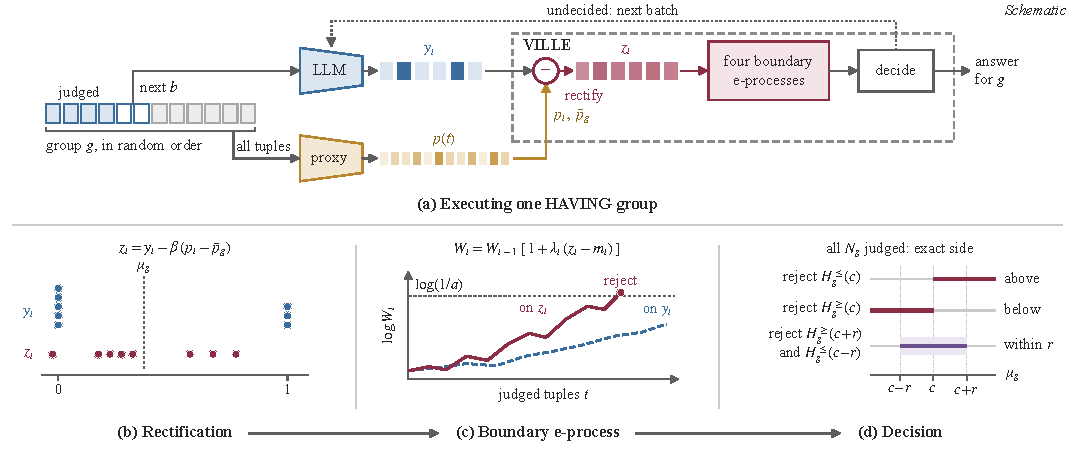
\includegraphics[width=\textwidth]{figures/overview_mechanism.pdf}
\caption{\sys{} executing one HAVING group. (a) In one random order, the LLM judges the next $b$ tuples, the proxy scores all tuples once, and \sys{} rectifies the judgments and updates four boundary e-processes until a decision is certified. (b) Rectification keeps the group mean $\mu_g$ for any proxy, and an informative proxy pulls 0/1 judgments toward it (eight tuples, $\beta=1$). (c) Each e-process bets against the remaining-population null mean $m_t$ (\Cref{eq:mt}) and rejects at wealth $1/a$, $a=\alpha/(2K)$; betting on $y_t$ (dashed) is slower. (d) Rejections that certify each answer; an exhausted group is decided exactly.}
\label{fig:overview}
\end{figure*}


\sys{} rests on three ideas.
First, it never estimates a group mean for its own sake; it tests only the few hypotheses that decide the answer (\Cref{sec:boundary}).
Second, each hypothesis is tested by a betting e-process, which stays valid under continuous monitoring and adaptive sampling (\Cref{sec:betting}).
Third, the e-process bets on proxy-rectified values, which keep the group mean intact while removing the variance that the proxy explains (\Cref{sec:rectify}).
\Cref{fig:overview} shows how the three fit together for one HAVING group.
\Cref{sec:wor,sec:pair} give the without-replacement forms for single groups and for pairs, and \Cref{sec:guarantee} states the guarantees.

\subsection{From decisions to boundary hypotheses}
\label{sec:boundary}

A decision query depends on the data only through a few comparisons.
For HAVING, group $g$ is answered by the outcome of four one-sided hypotheses:
\begin{equation}
\begin{aligned}
&H^{\le}_{g}(c):\mu_g\le c, && H^{\ge}_{g}(c):\mu_g\ge c,\\
&H^{\ge}_{g}(c+r):\mu_g\ge c+r, && H^{\le}_{g}(c-r):\mu_g\le c-r.
\end{aligned}
\end{equation}
Rejecting $H^{\le}_g(c)$ certifies ``above'', rejecting $H^{\ge}_g(c)$ certifies ``below'', and rejecting both $H^{\ge}_g(c+r)$ and $H^{\le}_g(c-r)$ certifies $|\mu_g-c|<r$, in which case either answer is $r$-correct.
For a pair of groups $(i,j)$, the same four hypotheses are posed on the difference $\mu_i-\mu_j$ with boundaries $0$ and $\pm r$.
ORDER BY and Top-$k$ are assembled from pair outcomes (\Cref{sec:processing}).

This formulation exposes the null value and direction relevant to each decision.
\sys{} uses them to choose a gap-adaptive bet for each boundary (\Cref{eq:lambda}) and to test group differences directly (\Cref{sec:pair}).
Both our tests and the confidence-sequence baselines stop when a side or an indifference decision is certified. The experimental comparison measures the combined effects of the betting rule and the paired construction.

\subsection{Testing by betting}
\label{sec:betting}

Consider a stream $z_1,z_2,\dots$ in $[\ell,h]$ and a null hypothesis that bounds the conditional mean of each observation by $m_t$, i.e., $\E[z_t\mid\F_{t-1}]\le m_t$.
A gambler starts with wealth $W_0=1$ and, before seeing $z_t$, stakes a fraction $\lambda_t\ge 0$ chosen from the past:
\begin{equation}
W_t=W_{t-1}\bigl(1+\lambda_t(z_t-m_t)\bigr).
\label{eq:wealth}
\end{equation}
If $\lambda_t\le\kappa/(m_t-\ell)$ for a constant $\kappa<1$, the wealth stays positive.
Under the null, $\E[W_t\mid\F_{t-1}]\le W_{t-1}$, so $(W_t)$ is a nonnegative supermartingale, or \emph{e-process}~\cite{ramdas2023savi,shafer2021}.
By Ville's inequality~\cite{ville1939},
\begin{equation}
\Prb\bigl(\exists t:\ W_t\ge 1/a\bigr)\le a .
\label{eq:ville}
\end{equation}
Rejecting the null as soon as the wealth reaches $1/a$ therefore has type-I error at most $a$, no matter how often the wealth is inspected, when sampling stops, or how the system decides which group to sample next.
This is exactly the protection that continuous monitoring requires, and it is what fixed-sample intervals lack.

The betting fraction determines power, and we use an approximately growth-rate-optimal fraction in the spirit of aGRAPA~\cite{wsr2024betting}:
\begin{equation}
\lambda_t=\min\Bigl\{\max\Bigl\{\frac{\hat\gamma_{t}}{\hat\sigma^2_{t}+\hat\gamma_{t}^2},\,0\Bigr\},\ \frac{\kappa}{m_t-\ell}\Bigr\},\qquad \kappa=\tfrac12,
\label{eq:lambda}
\end{equation}
where $\hat\gamma_t$ is the predicted excess of $\E[z_t\mid\F_{t-1}]$ over $m_t$ and $\hat\sigma^2_t$ is a running variance estimate, both computed from $z_1,\dots,z_{t-1}$ with one pseudo-observation on the null boundary.
Any predictable choice keeps the guarantee; this one makes the log-wealth grow at roughly $\gamma^2/(2\sigma^2)$ per call when the true excess is $\gamma$ and the variance is $\sigma^2$.
A test therefore rejects after about
\begin{equation}
n\approx\frac{2\sigma^2\log(1/a)}{\gamma^2}
\label{eq:cost}
\end{equation}
calls.
\Cref{eq:cost} explains where \sys{} saves: decisions pay $1/\gamma^2$ only for groups near a boundary, and the variance $\sigma^2$ is the target of the next step.

\subsection{Proxy rectification}
\label{sec:rectify}

Let $\bar p_g=\frac1{N_g}\sum_{t\in g}p(t)$ be the mean proxy score of group $g$, which is computed exactly because proxies are cheap.
For a weight $\beta\in[0,1]$, define the \emph{rectified value}
\begin{equation}
z(t)=y(t)-\beta\bigl(p(t)-\bar p_g\bigr),\qquad t\in g .
\label{eq:rectify}
\end{equation}

\begin{lemma}[Rectification preserves the group mean]
\label{lem:unbiased}
For every proxy and every $\beta$, $\sum_{t\in g}z(t)=N_g\mu_g$.
\end{lemma}
\begin{proof}
$\sum_{t\in g}z(t)=\sum_{t\in g}y(t)-\beta\bigl(\sum_{t\in g}p(t)-N_g\bar p_g\bigr)=N_g\mu_g$.
\end{proof}

The population of rectified values has exactly the group mean that the query asks about, so every test of \Cref{sec:boundary} can be run on $z$ instead of $y$.
Rectified values are the control-variate form that BlazeIt uses for estimation~\cite{blazeit} and the rectifier of prediction-powered inference~\cite{ppi,avppi,ppevalues}; \sys{} places them inside boundary tests under sampling without replacement.
Their variance is $\mathrm{Var}_g(y)-2\beta\,\mathrm{Cov}_g(y,p)+\beta^2\mathrm{Var}_g(p)$.
For $\mathrm{Var}_g(p)>0$, the population-optimal coefficient in $[0,1]$ is $\beta_g^\star=\min\{1,\max\{0,\mathrm{Cov}_g(y,p)/\mathrm{Var}_g(p)\}\}$.
When the unconstrained optimum lies in this interval, its variance is $(1-\rho_g^2)\mathrm{Var}_g(y)$, where $\rho_g$ is the correlation between the LLM judgment and the proxy.
At this ideal coefficient, \Cref{eq:cost} suggests roughly twofold and fivefold call savings at $\rho=0.71$ and $\rho=0.89$. Our implementation estimates a shared coefficient from an independent training set, and its variance follows the quadratic expression above.
A useless proxy gives $\rho=0$ and leaves the variance unchanged at $\beta=0$; even a misleading proxy only enlarges the variance.
Because \Cref{lem:unbiased} holds for every proxy, proxy quality affects cost and never validity.
We fix $\beta$ before the query from the small labeled set used to train the proxy; any data-independent $\beta$ is valid.

Rectification widens the range of the values: with $y,p\in[y_{\min},y_{\max}]$, the rectified values of group $g$ lie in $[\ell_g,h_g]=[y_{\min}-\beta(y_{\max}-\bar p_g),\ y_{\max}-\beta(y_{\min}-\bar p_g)]$, up to twice the original width.
Range-based bounds such as Hoeffding's pay for this growth in full.
The betting fraction in \Cref{eq:lambda} adapts to the variance and touches the range only through the cap, so \sys{} keeps most of the variance reduction.

\subsection{Sampling without replacement}
\label{sec:wor}

A tuple is judged at most once, so the tuples of a group are drawn without replacement: \sys{} draws a uniformly random permutation of group $g$ and judges its prefix.
Let $S_{t-1}=\sum_{s<t}z_s$ be the sum of the first $t-1$ rectified values.
Under without-replacement sampling,
\begin{equation}
\E[z_t\mid\F_{t-1}]=\frac{N_g\mu_g-S_{t-1}}{N_g-t+1}.
\end{equation}
Hence, under $H^{\le}_g(m)$, the conditional mean of the $t$-th draw is at most
\begin{equation}
m_t=\frac{N_g m-S_{t-1}}{N_g-t+1},
\label{eq:mt}
\end{equation}
which is the null value to plug into \Cref{eq:wealth}.

\begin{proposition}[One-sample test]
\label{prop:one}
Draw group $g$ without replacement and run \Cref{eq:wealth} on $z$ with $m_t$ from \Cref{eq:mt}, $\lambda_t$ predictable and $0\le\lambda_t\le\kappa/(m_t-\ell_g)$ with $\kappa<1$, $\lambda_t=0$ when $m_t\ge h_g$, and immediate rejection when $m_t<\ell_g$.
Then, under $H^{\le}_g(m)$, $\Prb(\exists t:\text{reject})\le a$.
\end{proposition}
\begin{proof}
Under the null, $\E[z_t\mid\F_{t-1}]\le m_t$ by \Cref{lem:unbiased} and \Cref{eq:mt}, so the wealth is a nonnegative supermartingale and \Cref{eq:ville} applies.
If $m_t<\ell_g$, the remaining $N_g-t+1$ values would have to average below their minimum, which contradicts the null, so the immediate rejection is never an error.
\end{proof}

The finite-population form matters in practice: as the prefix grows, $m_t$ moves away from $m$ whenever the observed values disagree with the null, and once every tuple has been judged the test decides with certainty.
Small groups, which with-replacement analyses treat as infinite, are certified well before exhaustion.
The upper hypothesis $H^{\ge}_g(m)$ is tested by applying \Cref{prop:one} to $-z$.

\subsection{Paired tests for orderings}
\label{sec:pair}

Orderings compare two groups whose sizes differ, often by orders of magnitude.
We draw one tuple from each group per step and use the per-draw statistic
\begin{equation}
u_{g,t}=\frac{(N_g-t+1)\,z_{g,t}+S_{g,t-1}}{N_g},
\label{eq:u}
\end{equation}
which satisfies $\E[u_{g,t}\mid\F_{t-1}]=\mu_g$ for every $t\le N_g$ by \Cref{sec:wor}.
Once a group is exhausted its mean is known, and we set $u_{g,t}=\mu_g$ for $t>N_g$.
For a pair $(i,j)$, the statistic $X_t=u_{i,t}-u_{j,t}$ has conditional mean exactly $\mu_i-\mu_j$, whatever the two group sizes.
Its bounds $\underline{x}_t$ and $\overline{x}_t$ follow from \Cref{eq:u} with $(z_{i,t},z_{j,t})=(\ell_i,h_j)$ and $(h_i,\ell_j)$ and are known before the draw.

\begin{proposition}[Paired test]
\label{prop:pair}
Let the two groups be sampled independently without replacement, and bet on $X_t-d$ as in \Cref{eq:wealth} with $\lambda_t$ predictable and $0\le\lambda_t\le\kappa/(d-\underline{x}_t)$ with $\kappa<1$, $\lambda_t=0$ when $\overline{x}_t\le d$, and immediate rejection when $\underline{x}_t>d$.
Then, under $H:\mu_i-\mu_j\le d$, $\Prb(\exists t:\text{reject})\le a$.
\end{proposition}
\begin{proof}
$\E[X_t-d\mid\F_{t-1}]=\mu_i-\mu_j-d\le0$ under $H$, and $1+\lambda_t(X_t-d)\ge1-\kappa>0$, so the wealth is a nonnegative supermartingale and \Cref{eq:ville} applies.
If $\underline{x}_t>d$, then $\mu_i-\mu_j=\E[X_t\mid\F_{t-1}]>d$, so the immediate rejection is never an error.
\end{proof}

Testing the difference directly saves calls: comparing two confidence intervals requires both of them to clear the gap, so their widths add, whereas the paired test pays once for the standard deviation of the difference.

\subsection{Guarantees}
\label{sec:guarantee}

Each decision is guarded by the boundary tests of \Cref{sec:boundary}, each run at level $a$.
Whatever the value of $\mu_g$, at most two of the four hypotheses of a group are true: $H^{\ge}_g(c)$, and $H^{\ge}_g(c+r)$ if $\mu_g\ge c+r$, when $\mu_g>c$; symmetrically when $\mu_g<c$; and $H^{\le}_g(c)$ and $H^{\ge}_g(c)$ when $\mu_g=c$.
The same holds for the four hypotheses of each of the $P=K(K-1)/2$ pairs.

\begin{theorem}[Certified decisions]
\label{thm:main}
Run the HAVING tests at $a=\alpha/(2K)$ and the pair tests at $a=\alpha/(2P)$.
For every data instance, every proxy, every fixed $\beta$, and every stopping rule and sampling schedule that depends only on past observations, the probability that \sys{} returns an answer that is not $r$-correct (\Cref{def:rcorrect}) is at most $\alpha$.
\end{theorem}
\begin{proof}
Conceptually, \sys{} fixes a random permutation of every group before the first call, and the schedule and stopping rule only decide how long a prefix of each permutation is read.
The wealth of a test after $t$ steps is a function of the first $t$ elements of the permutations it reads, and its bets depend on the first $t-1$.
By \Cref{prop:one,prop:pair}, a test of a true null therefore reaches $1/a$ at some step of the full permutations with probability at most $a$, and reading only a prefix cannot raise this probability.
Since at most two hypotheses per group or pair are true, the union bound shows that, with probability at least $1-2Ka=1-\alpha$ for HAVING and $1-2Pa=1-\alpha$ for orderings, no test ever rejects a true null.
On this event the answer is $r$-correct.
HAVING: a group certified above has $\mu_g>c$, one certified below has $\mu_g<c$, one certified as indifferent has $|\mu_g-c|<r$, and an exhausted group is decided exactly.
Top-$k$: if $S$ contained $i$ with $\mu_i<\mu_{(k)}-r$, some $j\notin S$ among the true top $k$ would have $\mu_j>\mu_i+r$, yet \sys{} returns $S$ only after resolving $(i,j)$ as ``$i$ ahead'' or ``tie'', and either outcome rejects a true null.
ORDER BY: if $\mu_i\ge\mu_j+r$, the pair is resolved as ``$i$ ahead'', and every group $k$ that $j$ beats has $\mu_k<\mu_j$, hence $\mu_i-\mu_k>r$, so $i$ beats $k$ too.
Thus $i$ wins strictly more pairs than $j$ and is ranked ahead of it (\Cref{sec:processing}).
\end{proof}

The guarantee needs no distributional assumption beyond the boundedness of the judgments and uniform sampling within groups.
It also covers the analyst or agent who watches the answer and stops early, because stopping is just another data-dependent rule.
Every group terminates: either a test fires, or all tuples are judged and the decision is exact.
